\section{Game Design, Prototype, and Testing}

\subsection{Design and Storyboard}
An initial storyboard of the first level, as well as the main concept
for the game, is shown in Figure~\ref{fig:storyboard}. The game centers around
one loop, in which the Player, or Players, attempt to escape an island that
they are told is inescapeable. In each loop, each Player must complete tasks
in order to keep the boat moving towards a distant island, such as maneuvering
the sail to increase speed in changing winds, or repairing damage from
cannonballs or collisions with rocks. Progress within the level is shown to the
Players, and the ``score'' is dependent on how long the ship stays afloat. The
level ends when the Players either arrive at the island or sink. Levels are
intended to be repeatable, with hazards spawning randomly to increase
replayability, allowing Players to play in a Party Game style. Points earned
in each run can be used to unlock new upgrade to survive longer or in harder
levels, as well as non-functional upgrades such as new hats. 

\begin{figure}[htbp]
    \centerline{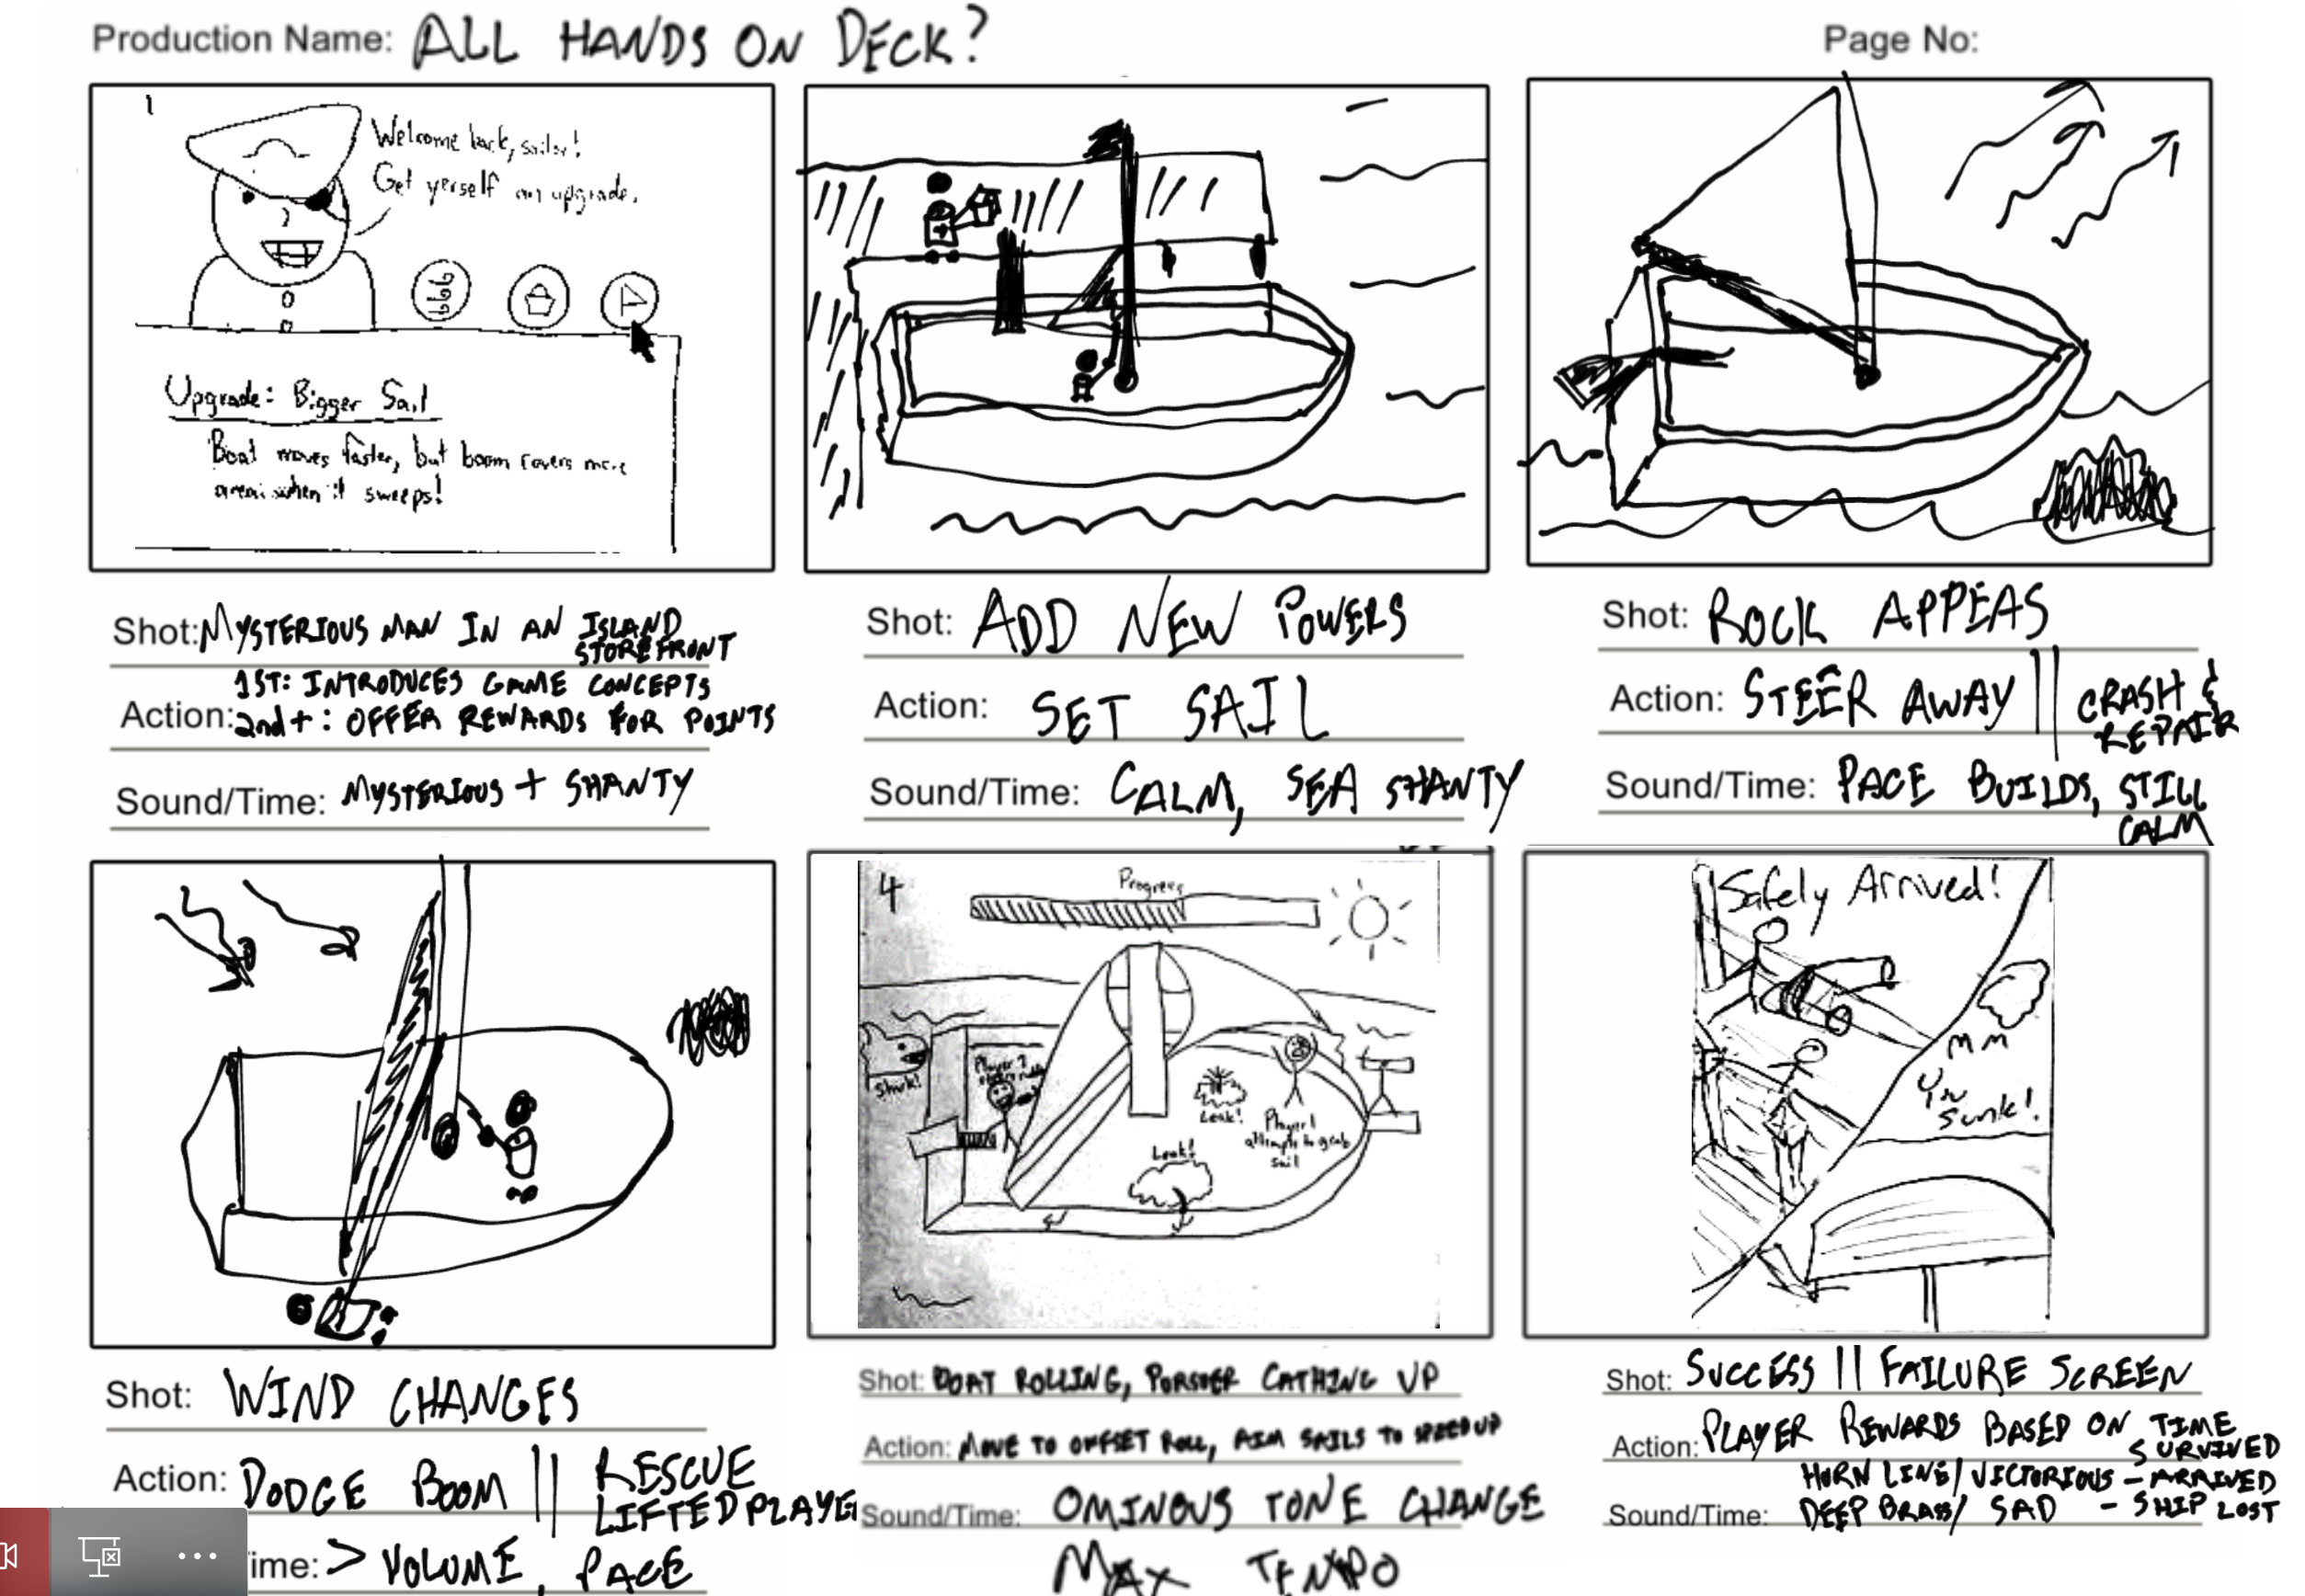
\includegraphics[scale=0.1]{figures/storyboard.png}}
    \caption{Storyboard of Level 1}
    \label{fig:storyboard}
\end{figure}

\subsection{Prototyping}
In order to test the concept of the main game loop, a prototype was developed
for play-testing, shown in Figure~\ref{fig:prototype}. Several of the original
features from the initial storyboard concept were implemented, including
randomly spawning rock and cannon hazards, a fully sailable ship with
maneuverable sail and rudder, \ac{UI}, and a game loop featuring initial story
beats with updating interactions based on whether the Players sunk or completed
the level.

\begin{figure}[htbp]
    \centerline{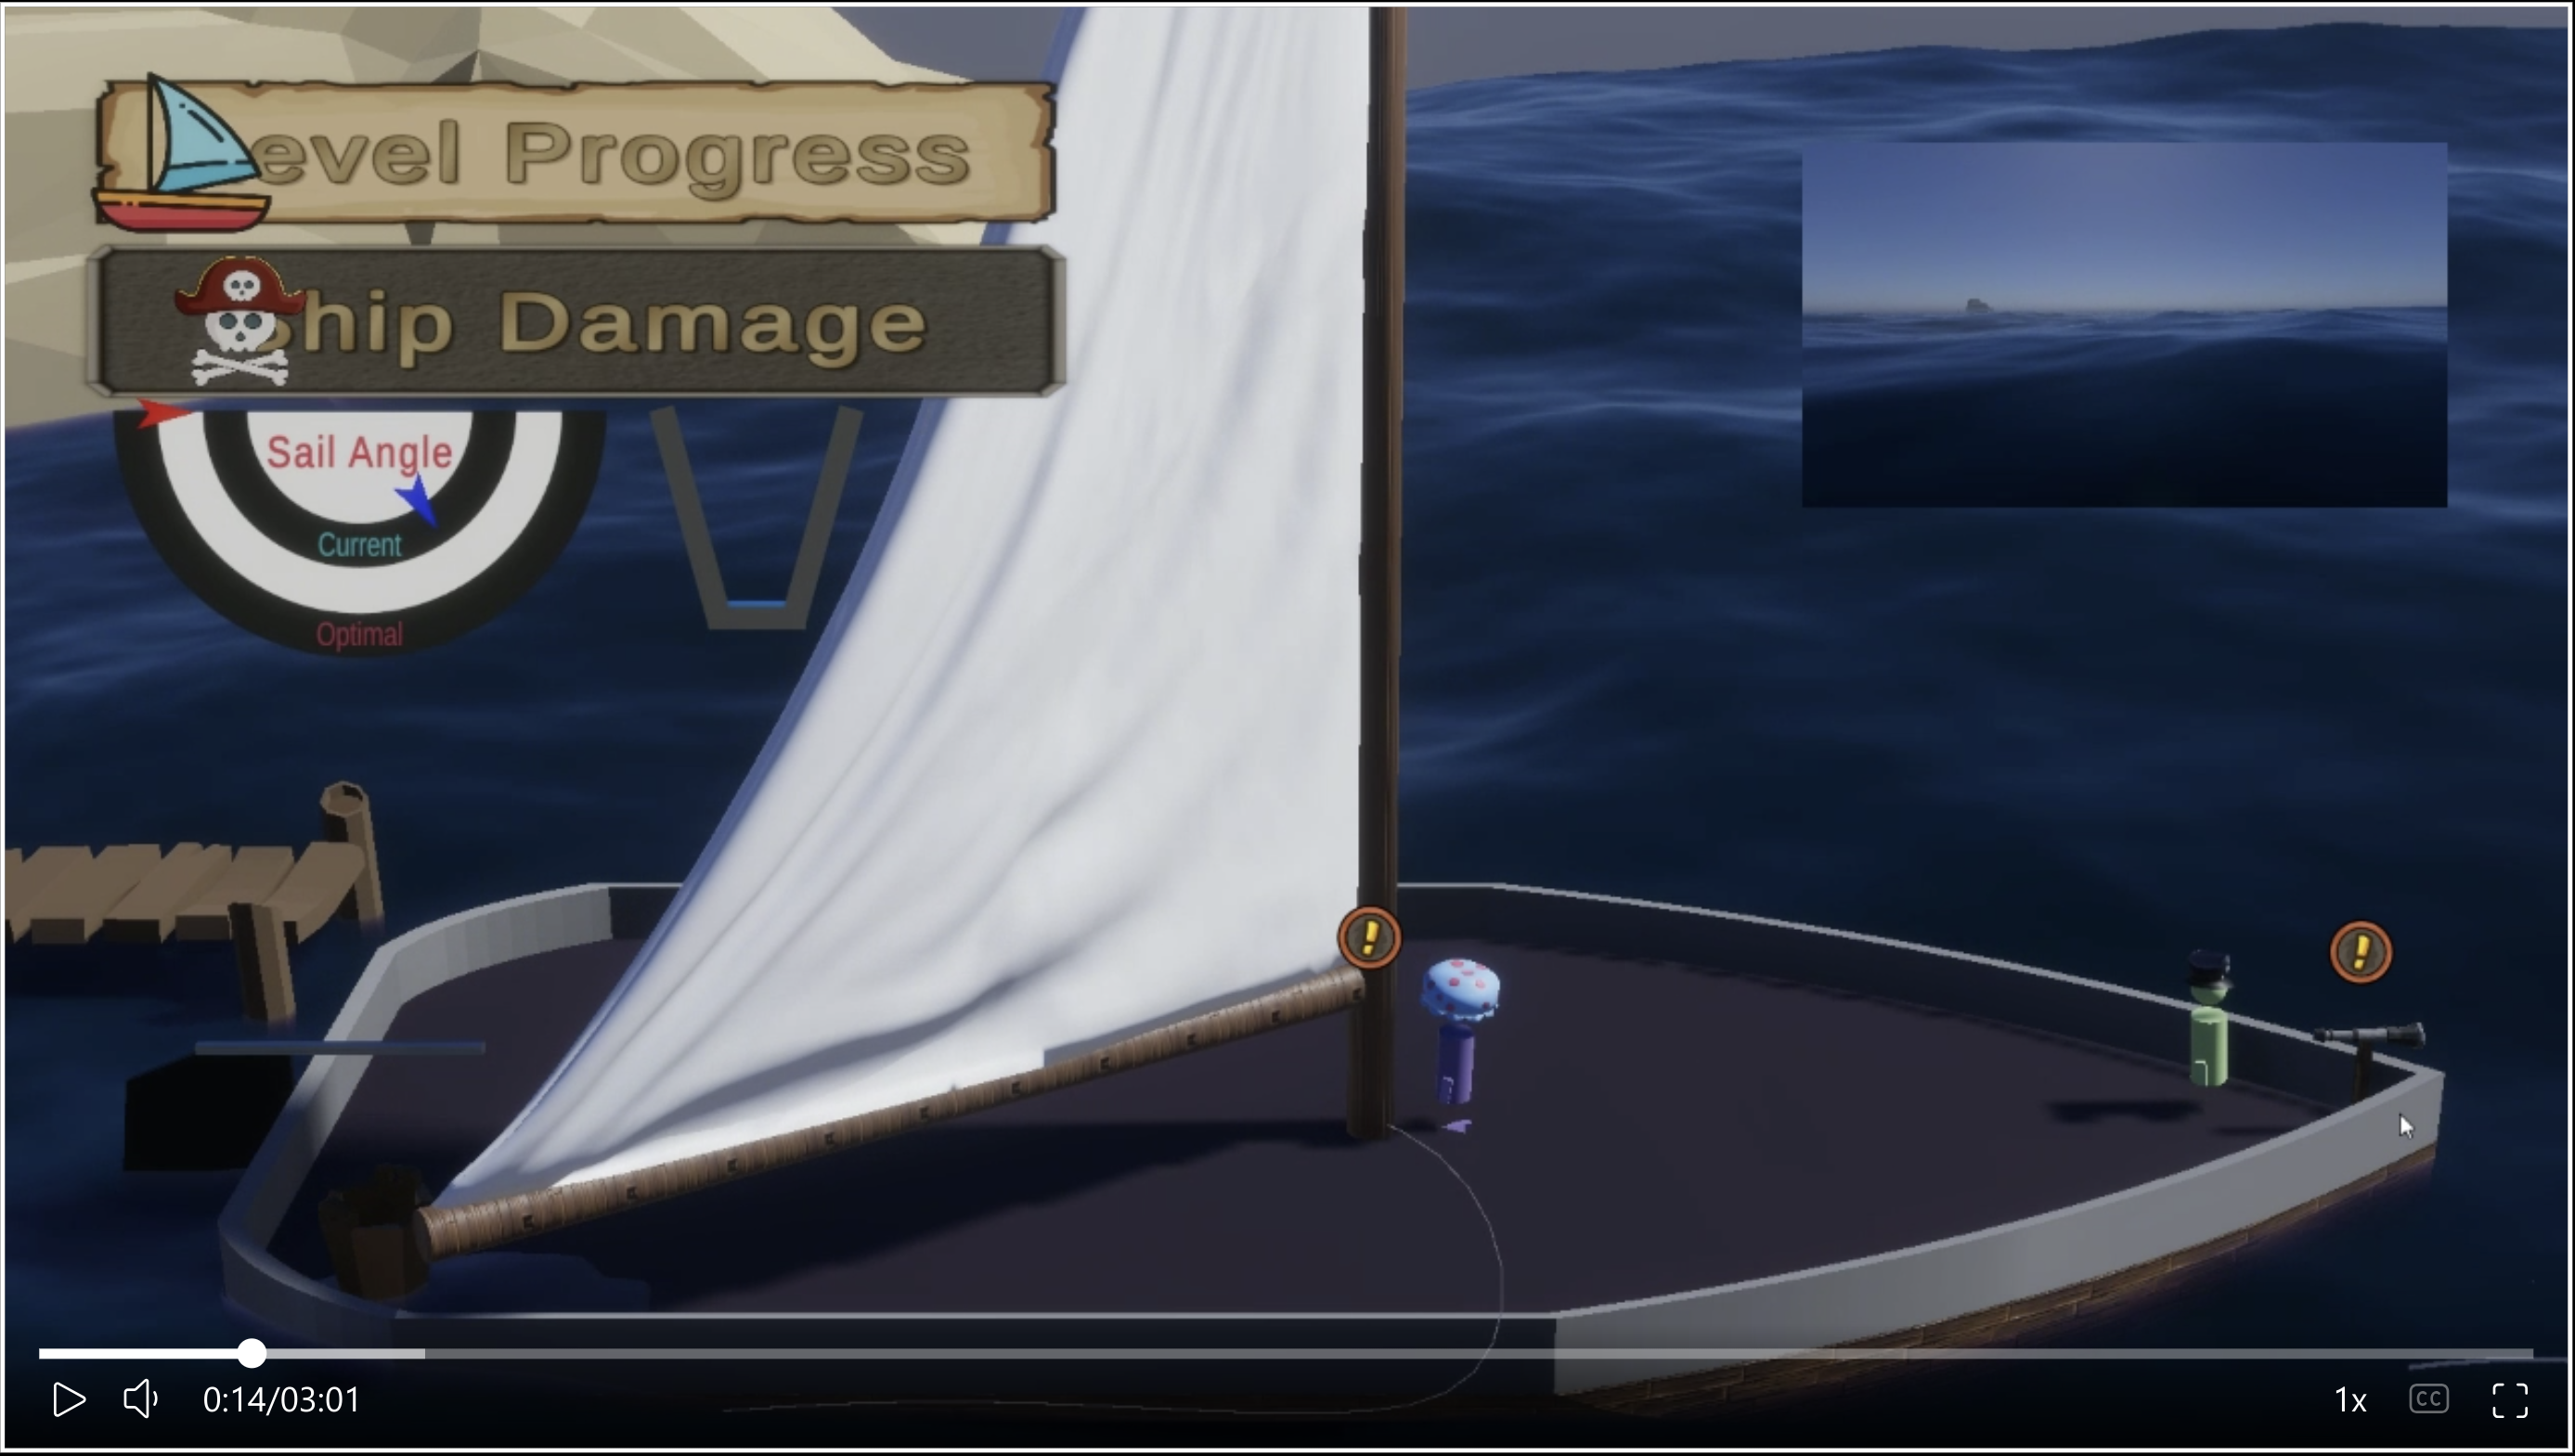
\includegraphics[scale=0.09]{figures/prototype.png}}
    \caption{Prototype of Level 1}
    \label{fig:prototype}
\end{figure}

\subsection{Play Testing}
With the initial prototyping complete, initial play tests were conducted. To
verify the viability of the game loop, the test plan includes tracking two
metrics: play time, and discrete Player feedback. For play time, the test will
track whether the game testers play for more than 4 minutes, which corresponds
to the playtime required to complete the initial test level. For discrete
feedback, developers will ask Players for any specific feedback on the game,
and track whether this feedback aligns with the plan for game development. If
feedback is in a alignment with future development plans, this is a good
indication that Player concerns are with prototype work and not issues game
design choices.
